\documentclass{esannV2}
\usepackage[dvips]{graphicx}
\usepackage[latin1]{inputenc}
\usepackage{amssymb,amsmath,array}
\usepackage{float}
\usepackage{subfig}

\newcommand\independent{\protect\mathpalette{\protect\independenT}{\perp}}
\def\independenT#1#2{\mathrel{\rlap{$#1#2$}\mkern2mu{#1#2}}}
\def\giv{\; | \;} % Given (|)
\def\ci{\independent}
\def\dep{\not\independent}

%***********************************************************************
% !!!! IMPORTANT NOTICE ON TEXT MARGINS !!!!!
%***********************************************************************
%
% Please avoid using DVI2PDF or PS2PDF converters: some undesired
% shifting/scaling may occur when using these programs
% It is strongly recommended to use the DVIPS converters, and to submit
% PS file. You may submit a PDF file if and only if you use ADOBE ACROBAT
% to convert your PS file to PDF.
%
% Check that you have set the paper size to A4 (and NOT to letter) in your
% dvi2ps converter, in Adobe Acrobat if you use it, and in any printer driver
% that you could use.  You also have to disable the 'scale to fit paper' option
% of your printer driver.
%
% In any case, please check carefully that the final size of the top and
% bottom margins is 5.2 cm and of the left and right margins is 4.4 cm.
% It is your responsibility to verify this important requirement.  If these margin requirements and not fulfilled at the end of your file generation process, please use the following commands to correct them.  Otherwise, please do not modify these commands.
%
\voffset 0 cm \hoffset 0 cm \addtolength{\textwidth}{0cm}
\addtolength{\textheight}{0cm}\addtolength{\leftmargin}{0cm}

%***********************************************************************
% !!!! USE OF THE esannV2 LaTeX STYLE FILE !!!!!
%***********************************************************************
%
% Some commands are inserted in the following .tex example file.  Therefore to
% set up your ESANN submission, please use this file and modify it to insert
% your text, rather than staring from a blank .tex file.  In this way, you will
% have the commands inserted in the right place.

\begin{document}
%style file for ESANN manuscripts
\title{Causal Relevance Learning for Robust Classification under Interventions}

%***********************************************************************
% AUTHORS INFORMATION AREA
%***********************************************************************
\author{Ernest Mwebaze$^{1,2}$ and John A. Quinn$^1$ and Michael Biehl$^2$
%
% Optional short acknowledgment: remove next line if non-needed
\thanks{We would like to acknowledge funding from NUFFIC NPT Project and Google Research Awards for this work.}
%
% DO NOT MODIFY THE FOLLOWING '\vspace' ARGUMENT
\vspace{.3cm}\\
%
% Addresses and institutions (remove "1- " in case of a single institution)
$^1$Faculty of Computing \& IT, Makerere University \\
P.O. Box 7062, Kampala, Uganda.%
% Remove the next three lines in case of a single institution
\vspace{.1cm}\\
$^2$ Johann Bernoulli Institute for Mathematics and Computer Science \\
Univ. of Groningen P.O. Box 407, 9700AK Groningen, The Netherlands\\
}
%***********************************************************************
% END OF AUTHORS INFORMATION AREA
%***********************************************************************

\maketitle

\begin{abstract}
In some classification problems the distribution of the test data is different from that of the training data because of external manipulations to the variables we observe. We propose a classification scheme which is robust to outside interventions by identifying causes in the training data, given that causes of a target variable remain predictive even when the data is manipulated. We do this be extending Relevance Learning Vector Quantization (RLVQ), a classification scheme that learns a relevance profile for the classification task presented. Our proposed algorithm, Causal-RLVQ, learns a relevance profile that weights causally relevant features more strongly. The algorithm can determines a tradeoff between robustness to intervention and accuracy on non-manipulated data, yielding RLVQ as a special case.
\end{abstract}

\section{Introduction}
\label{sec:Introduction}

Prototype based vector quantization schemes essentially operate by defining representatives (prototypes) in the data space. A dissimilarity measure, most commonly a distance based measure, is used to determine the dissimilarity between a data point and the prototype and hence perform the classification (or clustering) task. In this sense, Learning Vector Quantization (LVQ) and all its derivatives that are prototype based tend to be relatively easy to implement and provide classifiers that are intuitive to understand.

For our purposes here we look at Relevance Learning Vector Quantization (RLVQ)\cite{08} which introduces adaptive versions of the  dissimilarity measure based on how relevant the individual features in the data are for the classification task at hand. This has a two-fold advantage;(1) scaling the metric to fit the specific data hence improving classification and (2) introducing a feature selection or pruning algorithm. Like in most classification schemes, it is assumed the classifier will be used on a new dataset (test set) that has the same distribution as the dataset used for the training. Many real problems tend to violate this assumption because usually someone or some external factor has intervened on the new dataset. External factors could be artifacts due to the data collection process, or direct interventions for example one can imagine an economic status classification task where several interventions could significantly change the test set. 

In this paper we introduce a scheme that extends RLVQ to produce a causally relevant profile that will tend to offer more robust classification under such cases where the new data is suspected to have been intervened upon. We do this by trying to identify $V$-structures in the data and updating the relevance profile based on evidence we receive in the training of such a configuration amongst some of the features. This applies to the supervised learning LVQ schemes.

The structure of the remainder of the paper is as follows; initially we explain the problem of identifying causes from observational data, then give a small background on the basic RLVQ scheme that we extend in the following section. We then follow on with a description of how the causal relevance scheme works and we conclude with some experiments on different datasets.

\section{Identifying causes in observational data}
\label{sec:IdentifyingCausesInObservationalData}

Causation denotes that relationship between any two variables that entails that a change in one will influence a change in the other positively or negatively. Causal discovery by this definition hence necessitates an active process of intervening on one variable and determining if there is a corresponding change in the other one, an example being Randomized Control Experiments (RCE). This is however for most cases impractical or unethical and as such recent research in causality has focused on causal discovery purely from observational data. This is generally a daunting task and one has to be careful not to confuse correlation with causation, this leads to what is termed the classical paradoxes \cite{06}.

To discover causes from observational data, many of the methods todate use conditional independence(dependence) tests. $X$ is conditionally independent of $Y$ given $Z$, written $X \ci Y | Z$, if $P(X|Y,Z) = P(X|Z)$. 

\begin{figure}[!h]
	\centering
		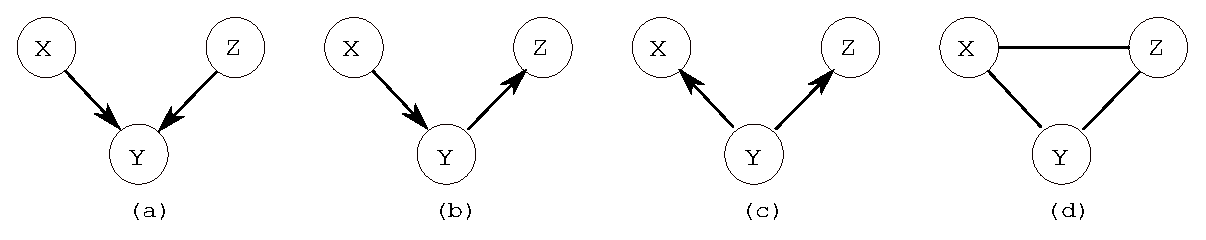
\includegraphics[width=0.80\textwidth]{vstructure.eps}
	\caption{Conditional independence configurations of 3 variables}
	\label{fig:vstructure}
\end{figure}

Figure \ref{fig:vstructure} shows the several conditional independence configurations of three variables $X,Y$ and $Z$ commonly identified as; (a) Collider: $X \ci Z$ but $X \dep Z | Y$, (b) Chain : $X \ci Z | Y$, (c) Fork : $X \ci Z | Y$, and (d) the fully connected configuration with indistinguishable conditional independence properties. Of these, the collider that provides the so-called 'V-structure' is of most critical importance in causal discovery because it is the only configuration that provides unique causal characteristics of the three. 

It suffices to note that most algorithms in causal discovery aim at discovering V-structures in the data as a way of determining causal relationships in the data. Causal discovery methods have also been extended in several ways including; using bayesian networks to model causal relationships using conditional independencies, search-and-score methods of causal discovery, causal discovery in multivariate relatinoships between continous variables using Structural Equation Models (SEMs), causal discovery using Independent Componenet Analysis and more recently progress has also been in discovering causality from cause-effect pairs \cite{15,14}.

\section{RLVQ}
\label{sec:RLVQ}

The basic LVQ scheme is set up as follows; Given a dataset $D = \left\{x^\mu, y^\mu\right\}^P_{\mu = 1}$ where $x^\mu \in R^N$ and the labels $y^\mu \in {1,2,\ldots C}$ correspond to one of the classes, the LVQ scheme is parameterized by a set of prototype vectors $W = \left\{w_j, c(w_j)\right\}^M_{j=1}$ with the prototype vectors $w_j$ having labels $c(w_j) \in {1,2,\dots C}$.

For a particular dissimilarity/distance measure $d(x,w)$, the LVQ classifier employs a Winner-Takes-All scheme where an arbitrary input is assigned to the class $c(W_L)$ of the closest prototype with $d(x,W_L) \leq d(x,w_j)$ \textsl{for all} $j$.

In the literature, many modifications of Kohonen's original formulation\cite{02} have been suggested with the aim of achieving better convergence and generalization behavior. A specific set of modifications have been towards accounting for heterogeneous datasets where features can have different meanings and magnitudes. These are the class of relevance learning schemes which employ adaptive scaling factors for each dimension in the feature space. A good background to these modifications is given elsewhere in the literature\cite{09,10,11}. For our purposes it will suffice to give the general formulation of RLVQ.

For RLVQ we can consider a generalized Euclidean distance of the form
%
\begin{equation} 
d(x,w_j) = \sum^N_{j=1} \lambda_j (x_j - w_j)^2 ,
\end{equation}
%
\noindent
as the dissimilarity measure where $\lambda_j$ are the adaptive relevance factors. The special case $\lambda_j = 1/N$ for all $j = 1,\ldots N$ is analogous to the original LVQ1 formulation. Each update of the winning prototype $w_j$ is accompanied by a corresponding update in the relevance factor $\lambda_j(t)$ as follows;
%
\begin{equation}
\lambda_j(t) = \lambda_j(t-1) - \eta_\lambda \phi (x_j - w_j)^2 
\end{equation}
%
\noindent
where $\lambda_j(t)$ is restricted to non-negative values and obeys the normalization $\sum^N_{j=1} \lambda_j = 1$.

The $\lambda$ update hence decreases the relevance factor $\lambda_j$ if the winning prototype $w_j$ does represent the correct class but the contribution $(x_j - w_j)^2$ to $d(x,w_j)$ is relatively large. Conversely the weight of a feature with relatively small $(x_j - w_j)^2$ is increased in such a case. The learning rates $\eta_w$ and $\eta_\lambda$ control the magnitude of the prototype and relevance factor updates at each step.

\section{CRLVQ}
\label{sec:CRLVQ}

CRLVQ is our extention of the RLVQ scheme where updates favor features that are causally related to the target feature. Our assessment of causal relevance is based on identifying V-structures with respect to the target. RLVQ gives a profile that represents how strongly each single dimension of the data is predictive of the target. In CRLVQ instead of looking at a single dimension, we look for evidence that there are two dimensions $x_i$ and $x_k$ that are predictive of the target. To ascertain that $x_i$ and $x_k$ are in a V-structure with the target we also check that they are independent of each other.

\begin{figure}[!h]
\begin{tabular}{m{.5\textwidth}cm{.4\textwidth}}
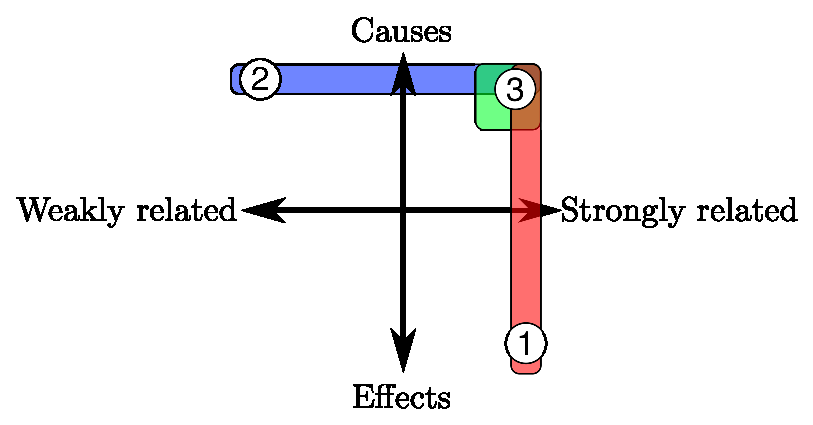
\includegraphics[width=.5\textwidth]{causal-relevance-dimensions.eps} & &
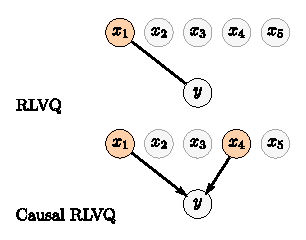
\includegraphics[width=.4\textwidth]{rlvq-crlvq.eps} \\
& \\
(a) & & (b)  
\end{tabular}
\label{fig:causes}
\caption{RLVQ and CRLVQ formulations. Panel (a) is an illustration of placement of variables across the predictive-causal space. Panel (b) shows how RLVQ is extended to CRLVQ}
\end{figure}

Figure 2 illustrates this salient distiction between RLVQ and CRLVQ. Panel (a) shows a placement grid for variables $(x_1, \ldots, x_P)$ categorised according to causal relevance or simply predictive relevance to the target variable $y$. Standard relevance learning aims to give higher weight to a set of variables (1) which are highly predictive; causal structure learning aims to find causes (2) or effects of a target; our work here identifies variables which are predictive causes (3). Panel (b) shows the criteria used for evaluating relevance scores in RLVQ and CRLVQ.
 
CRLVQ extends the RLVQ update by adding two extra evaluation criteria to equation 2. The three criteria in total are in a sense a distance-based formulation of the V-structure condition. For every example presented to the CRLVQ classification scheme, each component of $\lambda$ in CRLVQ is hence updated for every dimension $x_j$ for each introduction of a data example as follows
%
\begin{equation} 
\lambda_j(t) = \lambda_j(t-1) - \eta_\lambda \phi (x_j - w_j)^2 - \alpha \eta_\lambda \left( \min_{k \neq j}\left(\phi (x_k - w_k)^2 - (x_j - x_k)^2 \right) \right)
\end{equation}
%
The parameter $\alpha$ is a parameter that weights the two new criteria. Standard RLVQ is hence a special case of CRLVQ when $\alpha = 0$. We evaluate the independence of the different data dimensions by looking at their absolute difference. In z-transformed data, this will give a low number in the dimensions that are positively correlated. The update hence rewards any feature $x_j$ if it has a strong correlation(small difference) with the target/label vector $(x_j - w_j)^2$ , and also if there is strong evidence of another feature with a strong correlation to the target as well $(x_k - w_k)^2$, and if feature $x_j$ and $x_k$ are weakly correlated (large difference apart).

Note however that there might be other relationships between the dimensions that make them dependent on each other, but that this update would not capture for example negative correlation. 

\section{Experiments}
\label{sec:Experiments}

Simulated causal networks were used to validate the causal $\lambda$ update. One causal network was formulated as a 5-feature linear Gaussian network with 2 causes, 2 effects and 1 irrelevant feature.. 

\begin{figure}[!h]
\begin{tabular}{cc}
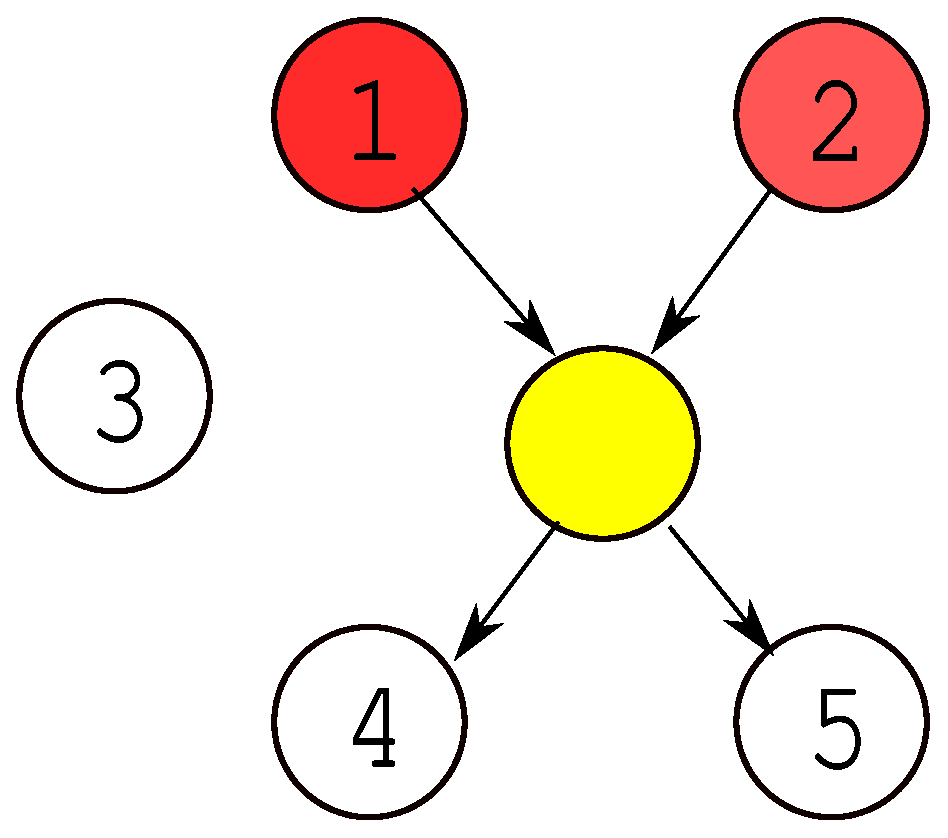
\includegraphics[scale=0.2]{simnetwork.eps} & 
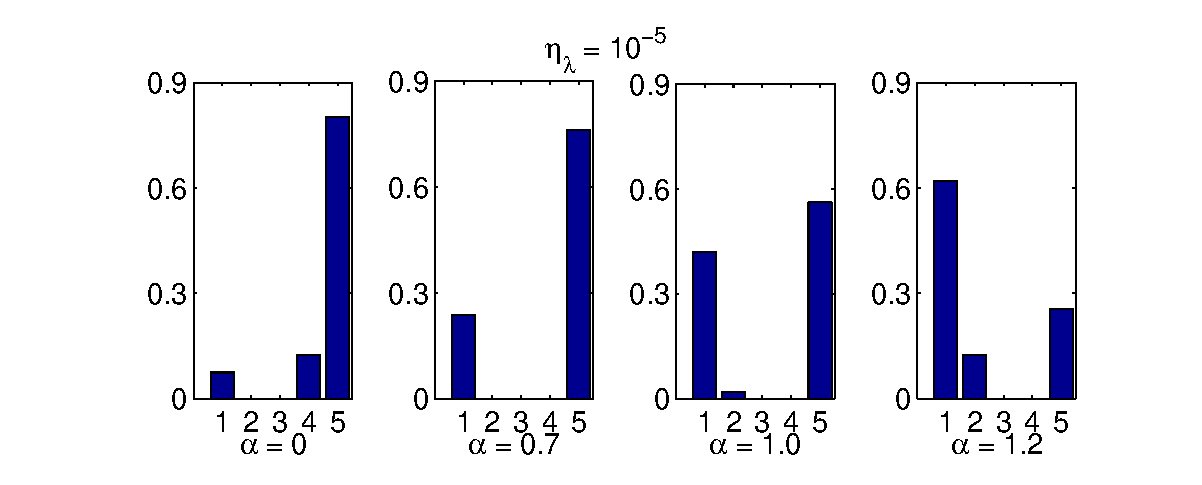
\includegraphics[width=.6\textwidth, height=.5\textwidth]{simlambda.eps} \\
(a) &  (b)  
\end{tabular}
\label{fig:simnetwork}
\caption{RLVQ and CRLVQ for Simulated Network. Panel (a) shows the simulated network with 2 causes, 2 effects and 1 irrelevant feature. Panel (b) shows the relevance profile under RLVQ and under CRLVQ for different parameter settings.}
\end{figure}

From Figure 3, it is evident to see that with introduction of the causal update, the learning favours the features that are causally relevant over the 'just' correlated features and the irrelevant or non-correlated features. Making the learning rate for the causal update bigger results in bigger updates in the learning as well.

For experiments on manipulated test sets we used a network simulated from a Bayes net and used for several causal competitions as a trial set for tuning causal algorithms. It is commonly called the Lucas dataset\cite{12} and tries to predict lung cancer based on different features. A full description of the dataset and its previous use can be found on the causality workbench\cite{13}. 3 versions of the dataset were used; Lucas0 - the natural network(unmanipulated) from which the training set was obtained, Lucas1 and Lucas2 - manipulated datasets of the same network from which the test data was obtained.

\begin{figure}[!h]
	\centering
		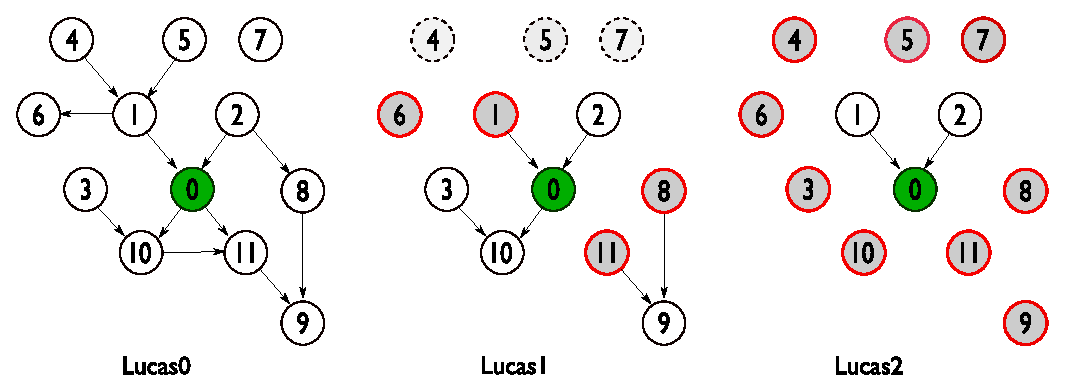
\includegraphics[width=1.0\textwidth]{lucasgraph.eps}
	\caption{\footnotesize{Lucas graphs showing the network structures for the unmanipulated set, Lucas0 and the manipulated sets, Lucas1 and Lucas2. The different features in the graphs are labelled as follows; 0 - Lungcancer, 1 - Smoking, 2 - Yellow Fingers, 3 - Anxiety, 4 - Peer Pressure, 5 - Genetics, 6 - Attention Disorder, 7 - Born an Even Day, 8 - Car Accident, 9 - Fatigue, 10 - Allergy, 11 - Coughing.}}
	\label{fig:lucasgraph}
\end{figure}

Figure \ref{fig:lucasgraph} illustrates the three networks from which the datasets were sampled. Networks for Lucas1 and Lucas2 show the features that were manipulated by setting them to arbitrary values. The effect of manipulations on a feature is to separate it from its parent features. Lucas1 had a few features manipulated while Lucas2 had all the features manipulated. The target was not manipulated. The network in Lucas2 represents an extreme case where all the features are manipulated, while this is unnatural, it illustrates the role of causes in classification when the data has been intervened upon because causes remain predictive and hence relevant for the classification.

\section{Results}
\label{sec:Results}

Table \ref{tab:TestErrorResults} shows the test error scores for the three datasets Lucas0, Lucas1 and Lucas2 for CRLVQ with varying $\alpha$ parameters. The first row with $\alpha$ = 0 represents RLVQ. Lucas0 represents the unmanipulated(natural) dataset while Lucas1 and Lucas2 represent manipulated/intervened upon datasets. Test results are obtained after 50 epochs through the data with $\eta_\lambda = 1e-6$.


\begin{table}
	\centering
			%\begin{footnotesize}
\begin{tabular}{|c|c|c|c|}
\hline
      &         \multicolumn{ 3}{|c|}{Lucas Dataset}   \\
\hline
$\alpha$ &  Lucas0 &     Lucas1 &     Lucas2  \\
\hline
  0    &    0.1820 &     0.1700 &     0.1800  \\
\hline
  0.3 &     0.1860 &     0.1680 &     0.1780  \\
\hline
  0.7 &     0.1860 &     0.1690 &     0.1780   \\
\hline
  1.0 &     0.1840 &     0.1680 &     0.1740   \\
\hline
  1.3 &     0.1850 &     0.1660 &     0.1740   \\
\hline
\end{tabular}   
			%\end{footnotesize}
	\caption{Test Error results for RLVQ and CRLVQ for the different datasets Lucas0, Lucas1 and Lucas2.}
	\label{tab:TestErrorResults}
\end{table}

For Lucas0, the unmanipulated dataset we notice a better test error for RLVQ ($\alpha = 0$) than for any other value of $\alpha$ (CRLVQ). This is plausible because for good classification performance effects (and possibly other features) are just as relevant as causes, so as we increase $\alpha$ we seive out most of the other features and keep the causally relevant features which may generally lead to poorer performance as is evidenced in the table.

For the manipulated datasets, Lucas1 and Lucas2 we notice the opposite effect. There is better accuracy as $\alpha$ is increased as expected because the causes remain predictive after the data is manipulated. A higher $\alpha$ biases the relevance profile towards causally relevant features hence the increase in performance. While generally this is true, the performance tends to be sensitive to the values of $\alpha$ and the RLVQ learning rate $\eta_\alpha$.

\section{Conclusion}
\label{sec:Conclusion}

This paper attempts to leverage techniques in causal learning and discovery and apply them to relevance learning for prototype-based classification. The goal is to assure robust classification when it is not certain that the test set has the same distribution as the training set, which is a common scenario in real applications. While our scheme is theoretically plausible, its actual formulation is still not very specific. This paper attempts a possible proof of concept and as such has several limitations in its present formulation; for example the scheme will only work if there are more than one cause and the causes are not related to each other. Also if causative cycles are present in the data, unreliable performance will result. 

The introduction of $\alpha$ is interesting because it can be tuned across a scale of RLVQ to CRLVQ and in a sense can depict the degree of certainty of manipulation of the test set. Presently this parameter is set arbitrarily, future work will look into how to learn this parameter as well. We also used a basic derivative of LVQ which has inherent problems in convergence and generalization of the classifier, however since CRLVQ mainly concerns how to update the relevance vector, we believe it can be easily extended to the different derivatives of LVQ including GRLVQ, GMLVQ and others. In future we will attempt to extend the update to these different schemes as well. Our formulation of the V-structures is not very specific and we have tried to highlight the short comings in different sections of this paper, in future providing a proper formulation will be one of our key concerns.

% ****************************************************************************
% BIBLIOGRAPHY AREA
% ****************************************************************************

\begin{footnotesize}

\bibliographystyle{unsrt}
\bibliography{esann2011}

\end{footnotesize}

% ****************************************************************************
% END OF BIBLIOGRAPHY AREA
% ****************************************************************************

\end{document}
